\documentclass{ws-ijbc}
\usepackage{ws-rotating}     % used only when sideways tables/figures are used
\usepackage{graphicx}
\usepackage{epstopdf}
\begin{document}

\catchline{}{}{}{}{} % Publisher's Area please ignore

\markboth{Author's Name}{Paper Title}

\title{Pictures with basic description\\
on \\
Kuramoto-Model Coupling Reconstruction Process}

\author{FIRST AUTHOR\footnote{Typeset names in 11 pt Times Roman.
Use the footnote to indicate the present or permanent address of
the author.}}

\address{University Department, University Name, Address\\
City, State ZIP/Zone, Country\\
fauthor@university.com\footnote{State completely without
abbreviations the affiliation and mailing address, including
country. Typeset in 11~pt Times Italic.}}

\author{SECOND AUTHOR}
\address{Group, Company, Address\\
City, State ZIP/Zone, Country\\
sauthor@company.com}

\maketitle

\begin{history}
\received{(to be inserted by publisher)}
\end{history}

\begin{abstract}
The abstract should summarize the context, content and conclusions
of the paper. It should not contain any references or displayed
equations. Typeset the abstract in 10~pt Times Roman with
baselineskip of 12 pt, making an indentation of 1.6~cm on the left
and right margins.
\end{abstract}

\keywords{A list of 3--5 keywords are to be supplied.}


\section{General scope of the reconstruction procedure and used notation}

In this part of the current paper we provide the description of Kuramoto
model, notation for used variables and general description of inverse
problem for Kuramoto model being studied.

Let us consider two oscillators with frequencies $\omega_{1}$ and
$\omega_{2}$ respectively; let $\Omega=\frac{\omega_{1}+\omega_{2}}{2}$
be their synchronized common frequency, thus 
\[
\begin{cases}
\omega_{1} & =\Omega+\Delta\omega\\
\omega_{2} & =\Omega-\Delta\omega
\end{cases},
\]
where we denote symmetrical frequency difference as $\Delta\omega$.
In order to describe the evolution of their phases $\theta_{1}(t)$
and $\theta_{2}(t)$ we propose following differential equations(let
us denote the coupling function of oscillators as $k=k(t)$):
\[
\begin{cases}
\dot{\theta}_{1}=\omega_{1}+\frac{k(t)}{2}\sin\left(\theta_{2}(t)-\theta_{1}(t)\right)\\
\dot{\theta}_{2}=\omega_{2}+\frac{k(t)}{2}\sin\left(\theta_{1}(t)-\theta_{2}(t)\right)
\end{cases},
\]
which could be easily transformed by summing and substracting equations
above into the following:
\[
\begin{cases}
\dot{\theta}_{1}+\dot{\theta}_{2}=2\Omega\\
\dot{\theta}_{1}-\dot{\theta}_{2}=2\Delta\omega-k(t)\sin\left(\theta_{1}(t)-\theta_{2}(t)\right)
\end{cases}
\]

Denoting $\theta=\theta_{1}-\theta_{2}$, we get 
\begin{equation}
\dot{\theta}=2\Delta\omega-k(t)\sin\theta(t)\label{eq:kur1}
\end{equation}
Solving equation (\ref{eq:kur1}), the evolution of phase difference
can be obtained (assuming the first equation of the system is easily
solvable); this states the direct problem in Kuramoto model.

Our paper focuses on the \emph{inverse} problem: considering that
the coupling $k(t)$ is generally unknown, let us assume that its
approximation $k_{0}(t)$ can be obtained from the real data (the
whole procedure of its extraction and necessary assumptions are discussed
in the third part of the paper). Then by solving equation (\ref{eq:kur1})
with $k=k_{0}(t)$ we get the approximation of phase difference $\theta_{0}(t)$;
this can be use to construct two ``virtual'' oscillators with given
phase difference $\theta_{0}(t)$ (assume $\theta_{1}(t)=\Omega t+\theta_{0}(t)/2$
and $\theta_{2}(t)=\Omega t-\theta(t)/2$ ):
\[
\begin{cases}
X_{0}(t)=\sin\left(\theta_{1}(t)\right)\\
Y_{0}(t)=\sin\left(\theta_{2}(t)\right)
\end{cases}
\]
Note that proposed virtual oscillators imply that amplitudes of both
oscillators are the same; moreover let us compute the sliding correlation
$C_{0}(t)$ between $X_{0}(t)$ and $Y_{0}(t)$ over a window of common
period of oscillators $T=\frac{2\pi}{\Omega}$:
\begin{align}
C_{0}(t) & =C_{T}(X_{0},Y_{0})=\label{eq:slide}\\
 & =\frac{\int_{t-T/2}^{t+T/2}\left(X_{0}(\tau)-\left\langle X_{0}(\tau)\right\rangle _{T}\right)\left(Y_{0}(\tau)-\left\langle Y_{0}(\tau)\right\rangle _{T}\right)d\tau}{\sqrt{\int_{t-T/2}^{t+T/2}\left(X_{0}(\tau)-\left\langle X_{0}(\tau)\right\rangle _{T}\right)^{2}d\tau\int_{t-T/2}^{t+T/2}\left(Y_{0}(\tau)-\left\langle Y_{0}(\tau)\right\rangle _{T}\right)^{2}d\tau}},\nonumber 
\end{align}
where by $\left\langle X_{0}(\tau)\right\rangle _{T}$ we denote the
mean value of $X_{0}(t)$ over used window.

The main assumption of overseen reconstruction procedure states that
the system is close to its stationary state; in which case the sliding
correlation between oscillators can be computed as $\theta_{0}(t)=\cos C_{0}(t)$.
Let us denote reconstructed phase difference in assumption of stationarity as $\varphi(t)$ which can be
obtained using $C_{0}(t)$ computed by equation (\ref{eq:slide}):
\[
\varphi(t)=\arccos C_{0}(t)
\]
Using that $\dot{\varphi}\approx0$ one could substitute $\theta$
with $\varphi$ in the equation (\ref{eq:kur1}) and find reconstructed
coupling $\hat{k}(t)$:
\[
\hat{k}(t)=\frac{2\Delta\omega}{\sin\varphi(t)}
\]

Note that described procedure is proven to be correct in case
\begin{equation}
\left|k_{0}(t)\right|\ge2\Delta\omega\label{eq:ineq}
\end{equation}

which is referred as \emph{the synchronization inequality}; this statement is sufficient but not necessary thus current paper investigates quality of described process focusing on the synchronization inequality breaking.

\section{Model functions and reconstruction}

In this part of our research we investigate the proposed reconstruction
procedure from qualitative and quantitative (we describe used metrics
further) points of view for 4 different sets of couplings
$k_{0}(t)$: piecewise-constant, sine, autoregressive approximations
and its combination; focusing on the case of temporarily breaking
the synchronization inequality (\ref{eq:ineq}).

\subsection{Piecewise-constant approximations}

In this case we assume that $k_{0}(t)$ can be described as
\[
k_{0}(t)=\begin{cases}
d, & t<T_{0}\lor t>T_{0}+s\\
d+\Delta d, & T_{0}\le t\le T_{0}+s
\end{cases}
\]
where $\Delta d$ can be either positive or negative; we refer to
the period of the second value $d+\Delta d$ as the shock period.

\begin{figure}[!h]
\centering{}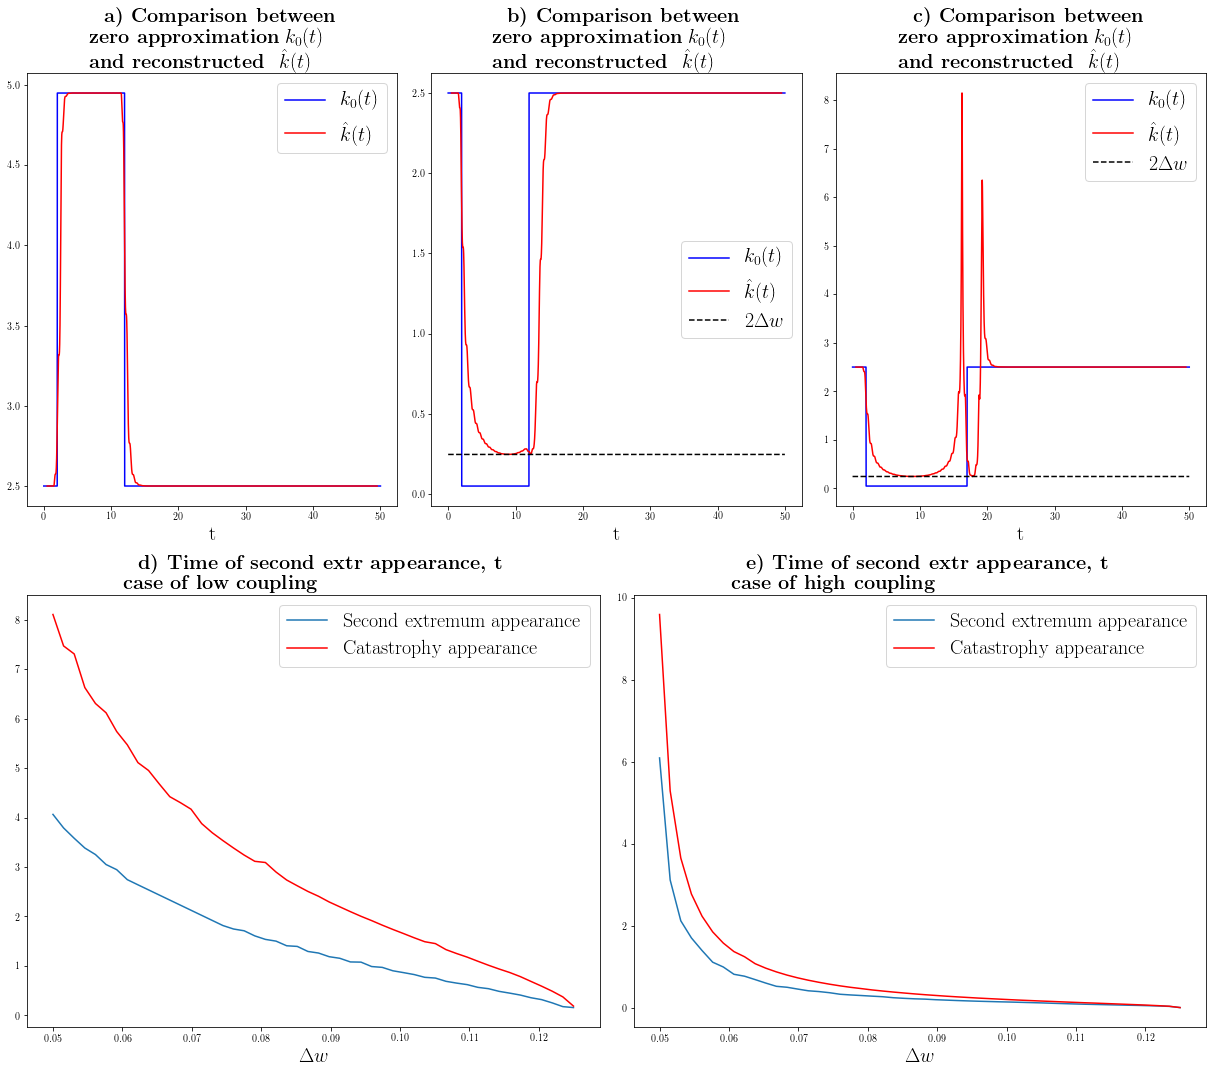
\includegraphics[width=1\textwidth]{../../../python/pics/v2/constv2}\caption{Reconstruction of piecewise-constant aprroxiamtion $k_{0}(t)$: examples
and length of the period with shock corresponding to the second extremum
and singularity appearances\label{fig:pc}}
\end{figure}

Figures (1a\textendash c) illustrate results of reconstruction of
single approximation in three different cases: without breaking the
synchronization inequality (1a); breaking Kuramoto inequality with
resulting additional extremum appearance after the shock period (1b);
and breaking Kuramoto inequality with resulting appearance of singularity
in reconstructed function (1c). 

In case of (1a) it can be seen that the system relaxes to the shocked
value during the shock period and to the normal value after the shock
significant amount of time (measured in common periods of oscillators);
thus one can say that the system has a noticeable ``memory''. As
for the effects of breaking the synchronization inequality (among
cases in which the shock period is not long enough to create qualitatively
new figures) we outline two different scenarious: if the shock period
is long enough (consider figures (1d\textendash e) in order to established
the appropriate length) reconstructed function tends to begin a relaxation
to the normal value even before the shock period is over thus creating
the second extremum after the shock; in case when the system has enough
time to fully relax to the normal value during the shock, the reconstruction
process results into the singularity in $\hat{k}(t)$ (specifically
this means that in that moment of time oscillators are fully uncorrelated). 

For the further investigation of this phenomena we provide figures
(1d\textendash e) devoted to establishing the length of the shock
period $s$ towards $\Delta\omega$ sufficient for the second extremum
and singularity; to give more sophisticated picture we study cases
of low coupling (low $d$, comparatively to $2\Delta\omega$) (fig.
1d) and high coupling (fig. 1e). As shown increasing (and therefore
strengthing the breaking difference in the inequality) symmetrical
phaze difference results into earlier appearance of both effects and
shorter time interval between the second extremum appearance and the
singularity.

\subsection{Sine approximations}

In this part we propose coupling approximation as follows:
\[
k_{0}(t)=A\sin\left(Bt+\varepsilon\right)+C,
\]

where $A$ is an amplitude, $B$ is a frequency and $C$ is a mean
value. Moreover, unless stated otherwise, consider $C-A<2\Delta\omega$,
so we study mainly the case of inequality breaking.

\begin{figure}[!h]
\centering{}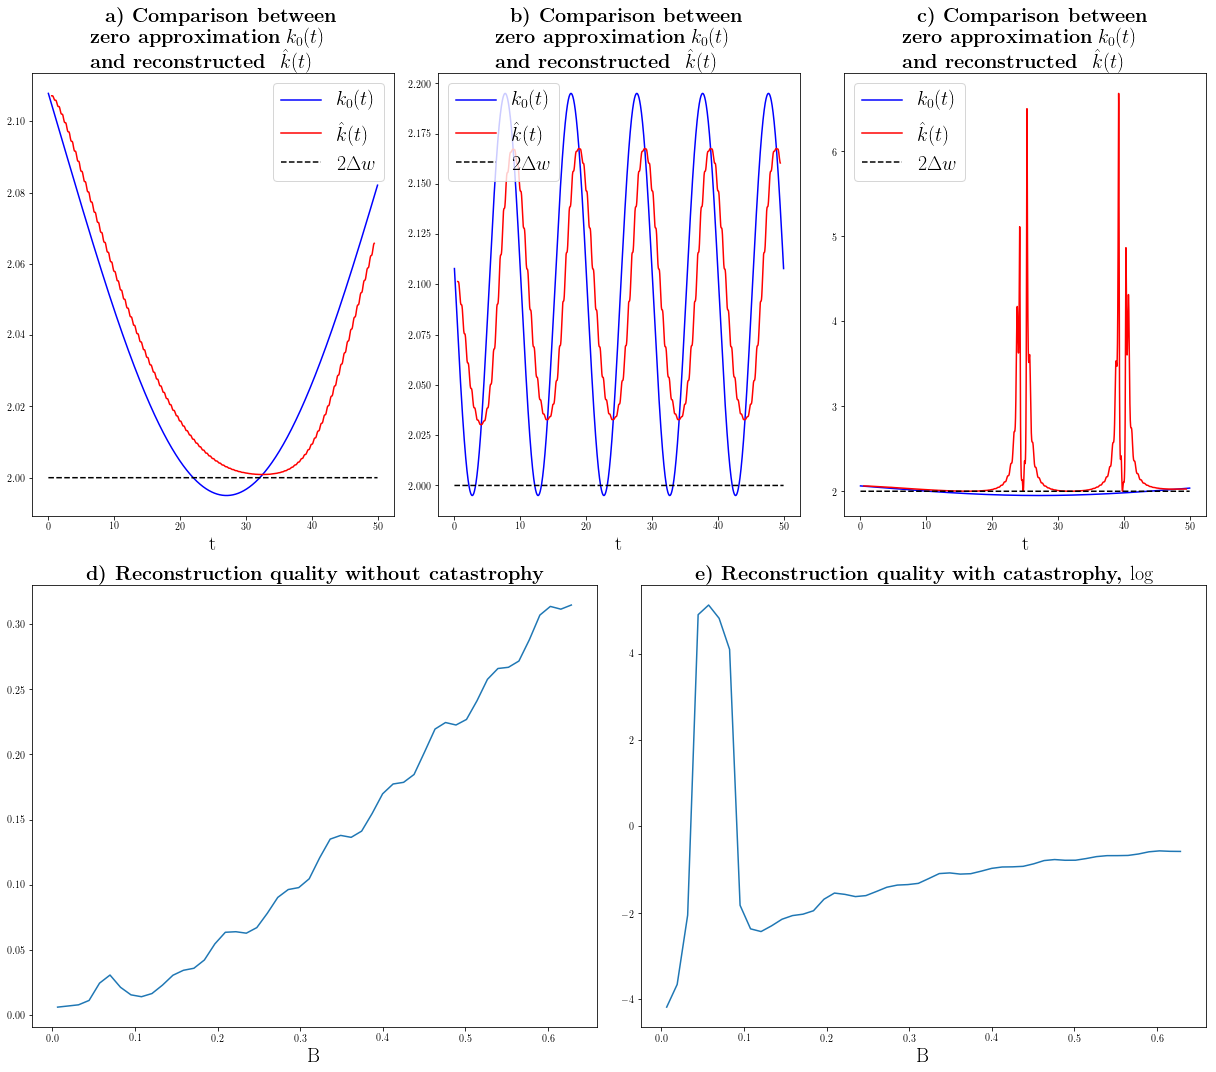
\includegraphics[width=1\textwidth]{../../../python/pics/v2/sinv2}\caption{Sine approximations of $k_{0}(t)$: examples and quality of reconstruction
towards sine frequency\label{fig:sin}}
\end{figure}

Same as for piecewise-constant case, figures (2a\textendash c) illustrate
results of reconstruction of single approximation; for those pictures
we vary the frequency of sine being reconstructed. Figure (2a) shows
the case for correct reconstruction despite the inequality breaking;
similar to the piecewise-constant case (fig. (1b)) we observe gradual
relaxation to values restricted by inequality with noticeable flattening.
Figures (2b) and (2c) shows two opposite cases of poor recontruction
quality: for the figure (2b) it can be seen that more frequent fluctuation
are less appropriate for the reconstruction which can be explained
by an absense of sufficient time for relaxation as seen on fig. (1)
and (2a); figure (2c) demonstates the case of singularity achieved
by the same condition as on fig. (1c) \textemdash{} too long restricted
value period.

Figures (2d\textendash e) generalize the study of reconstruction towards
approximation's sine frequency; to measure the quality of the process
we propose the following metric:
\[
R_{0}[\hat{k},k_{0}]=\frac{\int_{0}^{L}\left(k_{0}(t)-\left\langle k_{0}(t)\right\rangle _{L}\right)\left(\hat{k}(t)-\left\langle \hat{k}(t)\right\rangle _{L}\right)dt}{\int_{0}^{L}k_{0}^{2}(t)dt}
\]
(in assumption that $t\in[0;L]$ so $L$ denotes the end of time interval
being studied). Figure (2d) illustrates the case of $C-A>2\Delta\omega$;
thus general increase of error corresponds with phenomenon observed
on fig. (2b). Figure (2e) explores the case of $C-A<2\Delta\omega$
(in log scale): here we can see three different parts \textemdash{}
the first one corresponds to the case of no breaking (such as fig.
(2d)), then we obtain highly unreconstructed part corresponding to
fig. (2c) associated with singularities and finally we get similar
to fig. (2d) plot explained by increase of sine frequency.

\subsection{Autoregressive ramdom approximations}

In order to simulate the random noise for our procedure we study autoregressive
process (AR(1)), which can be described as:
\[
k_{0}(t_{n})=\alpha k_{0}(t_{n-1})+\xi_{n},
\]

where $\xi_{n}\sim\mathcal{N}(\mu,\sigma)$ and $0<\alpha<1$. This
stochastic process is widely on as weakly stationary after $n=\frac{1}{1-\alpha}$
with the mean equal to $\frac{\mu}{1-\alpha}$ and the standart deviation
equal to $\frac{\sigma^{2}}{1-\alpha^{2}}$.

\begin{figure}[!h]
\centering{}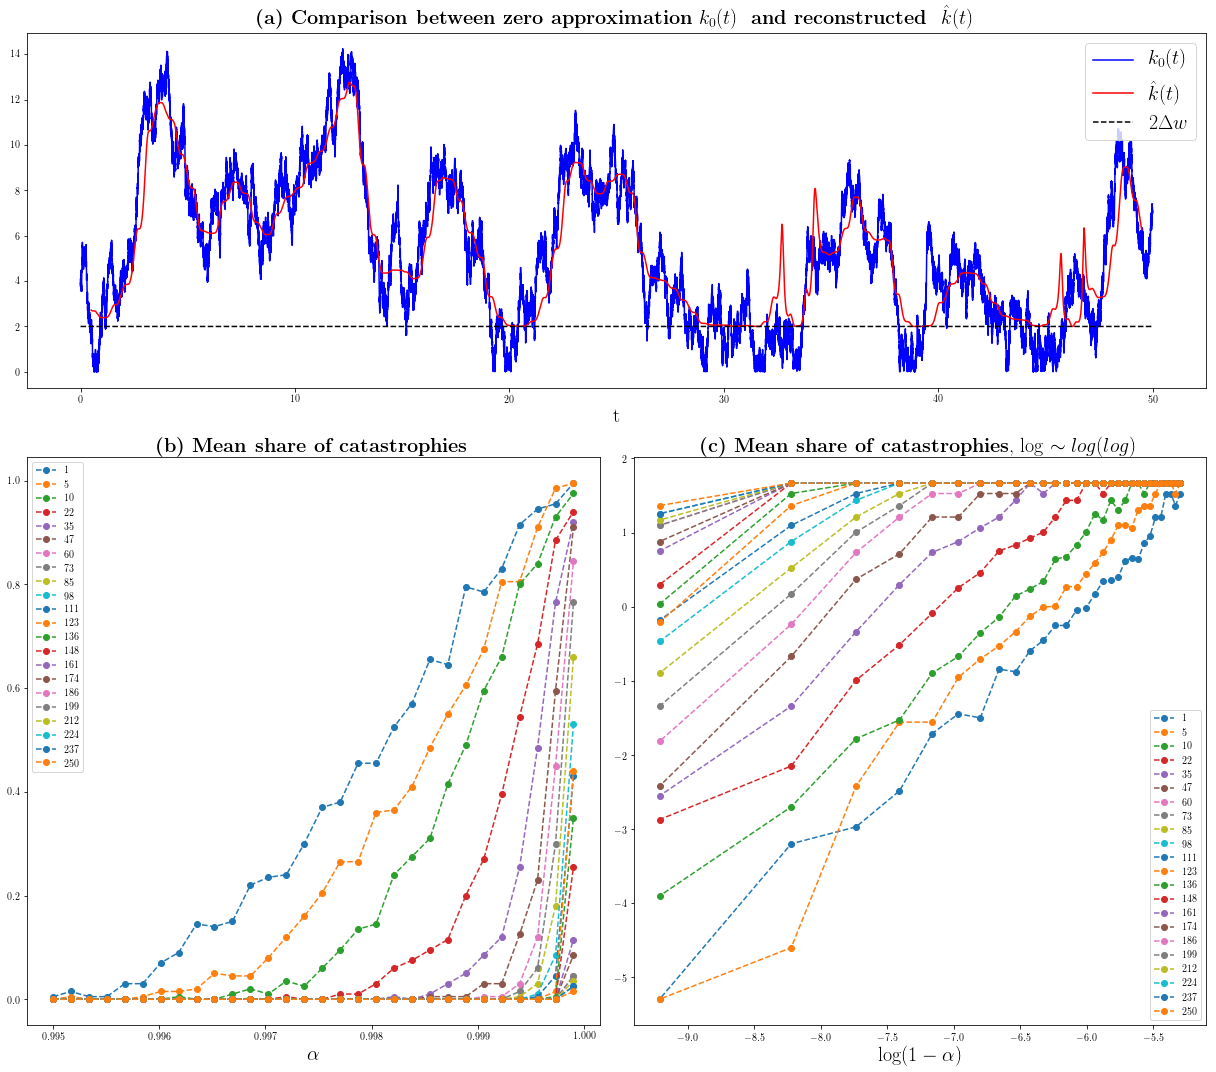
\includegraphics[width=1\textwidth]{../../../python/pics/v2/ar1v2}\caption{Autoregressive approximations of $k_{0}(t)$: an example and the probability
of singularity towards $\alpha$ and $\mu$ \label{fig:ar}}
\end{figure}

One realization of described process and its reconstruction are shown
on figure (3a); more precisely, in that case we obtain the general
understanding of reconstruction as smoothing highly variable approximations;
furthermore it can be seen that for the time interval in around $t\approx15$
we get poor reconstruction quality explained by rapid change of $k_{0}(t)$
as for too frequent sine series as in fig. (2b); for the time interval
in around $t\approx20$ we get a correct reconstruction with flattening
similar to fig. (2a); the time interval for $t\approx32$ illustrates
the occurence of singularity with the same reasoning as for piecewise-constant
and sine cases.

According to the stochasticity of the process one should assume that
for every set of parameters all seen for previous functions cases
of reconstruction are possible with some probability. Thus we vary
$\alpha$ and $\mu$ on figure (3b\textendash c) in order to get the
probability of singularity in each case (the mean $\mu=2\Delta\omega+K\sigma$
is varied through $K$). As shown on figure (3b) it can be concluded
that the probability of obtainig singularity through the reconstruction
declines with the mean growth which can be explained by the fact that
with the mean growth expected values of the stochastic process are
more distant from $2\Delta\omega$ with fixed variance; thus prolonged
restricted values of the process are less likely. Another trend of
figure (3b) is general growth of singularity probability towards $\alpha$;
specifically, as shown in figure (3c) in $\log X\sim\log\log Y$ scale,
it is linear with regression coefficient equal to 1 (with non-distinctive
fluctuations). One should notice that whilst being linear in $\log X\sim\log\log Y$
scale, given plot is not linear in simpler $X\sim\log Y$ scale; it
can be explained by the presense of pre-exponential functional factor
$f(\alpha)$ that gets close to constant only in $\log X\sim\log\log Y$
scale.

\subsection{Noised sine approximation and CIs}

The last family of model functions used as $k_{0}(t)$ approximation
is the combination of simple sine approximation with random additive
noise decribed above; precisely
\[
k_{0}(t)=A\sin(Bt+\varepsilon)+C+X(t_{n}),
\]
where $X(t_{n})=\alpha X(t_{n-1})+\xi_{n}$, $\xi_{n}\sim\mathcal{N}(0,\sigma)$,
$0<\alpha<1$.

\begin{figure}[!h]
\centering{}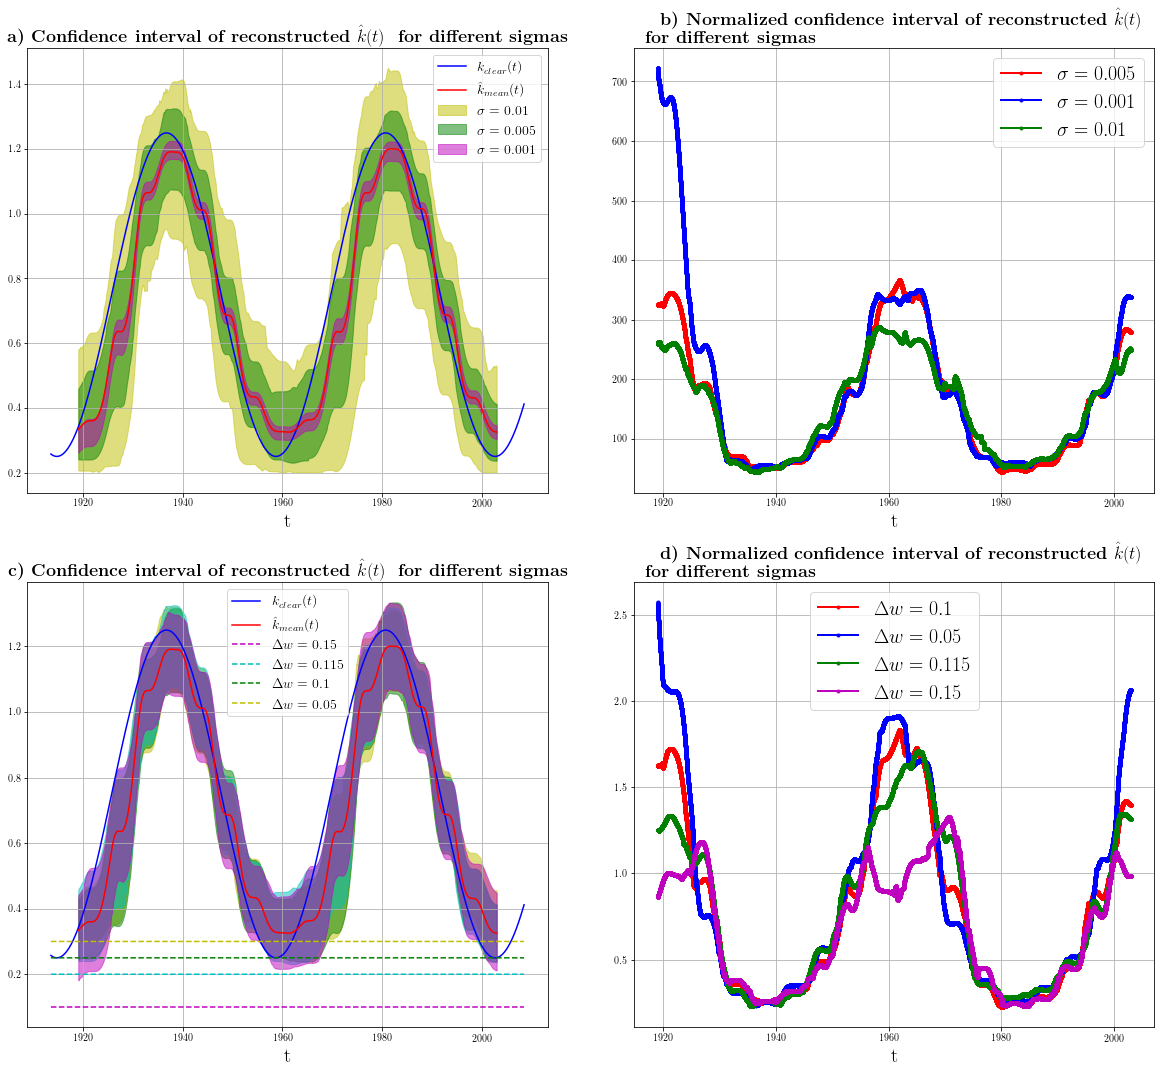
\includegraphics[width=1\textwidth]{../../../python/pics/v2/civ2}\caption{Sine approximations of $k_{0}(t)$ with additive autoregressive noise:
varying $\sigma$ and $\Delta\omega$\label{fig:ci}}
\end{figure}

In this scope for given problem the main question one should answer
is how influential the additive autoregression process is; in other
words we should establish the confidence interval associated with
random noise for reconstructed function $\hat{k}(t)$; let us denote
the width of the confidence interval as $e(t)$. For figures (4a,c)
we determine 95\% confidence interval for each moment of time (note
that there is no given knowledge about the distribution); also we
provide de-noised $k_{0}^{clear}(t)$ and $\hat{k}^{clear}(t)$ in
orde to illustrate centers of confidence interval and describe overall
reconstruction error.

Figures (4a\textendash b) demonstrates the case of varying $\sigma$in
additive noise; for each case figure (4b) shows the corresponding
plot $e(t)/\left(\sigma\cdot k_{0}^{clear}(t)\right)$. Therefore
it can be concluded that the width of confidence interval is proportional
to the noise's variance; in the same time plots discrepancies correspond
to lower phazes of the de-noised sine series where as seen on fig.
(3b) the probability of singularity occurence is higher thus making
reconstruction mostly incorrect and more variable. Figures (4c\textendash d)
compiled similarly to figures (4a\textendash b); note that in this
case we vary the Kuramoto inequality threshold $\Delta\omega$ and
since figure (4c) does not demonstrate any difference in confidence
intreval's widths towards the threshold, we use only $e(t)/k_{0}^{clear}(t)$
for figure (4d). Note that the case of $\Delta\omega=0.15$, which
implies not only random breaking of the synchronization inequality
but also systematical breaking as shown on figure (4c) with yellow
dashed line, noticeably differs from the others; despite the fact
that it is seemingly more probable case for singularity occurence,
the plot is lower than the others which can be explained by the fact
that not only we obtain singularity and incorrect reconstrucions but
we also obtain correct ones with flattening (as discussed earlier)
to $2\Delta\omega$ thus making reconstructed function less variable
resulting in more narrow confidence interval.
\end{document}
